
This Section will present the performance obtained when applying the strategies proposed in Section \ref{sec:cap_03}. The following will describe four different representative planning benchmarks, which will be employed later to show the computational times obtained applying the strategies proposed, when varying the number of threads.

\subsection{Problem 1 : path planning}
\label{sec:probl_1}

Here we consider a classical path planning problem. The robot adopted is a 3 d.o.f. robot with simplified shaped links. Every state $x \in X$ is simply the pose of the robot, i.e. the 3 values describing the angular joint displacements. The admissible region $\underline{X}$ is represented by the free configurational  space, i.e. the set of poses $x$ for which the robot is not in collision w.r.t. all the fixed obstacles populating the scene. The workspace of the robot is represented in Figure \ref{fig:Problem_1}.
An optimal trajectory $\tau_{1 \rightarrow 2}$ is the segment in the joint space whose extremals are $x_{1,2}$, and the length of such segment is considered as $C(\tau_{1 \rightarrow 2})$.
The states $x^k_s$ are obtained  by following the segment connecting $x_{Nearest}$ to $x_{target}$ with a fixed length step $l$ (apriori decided):
\begin{eqnarray}
L &=& l \cdot \frac{x_{target}-x_{Nearest}}{\Vert x_{target}-x_{Nearest} \Vert} \nonumber\\
x^k_s &=& x_{Nearest} + k \cdot L
\end{eqnarray}

\begin{figure}
	\centering
\subfloat[]{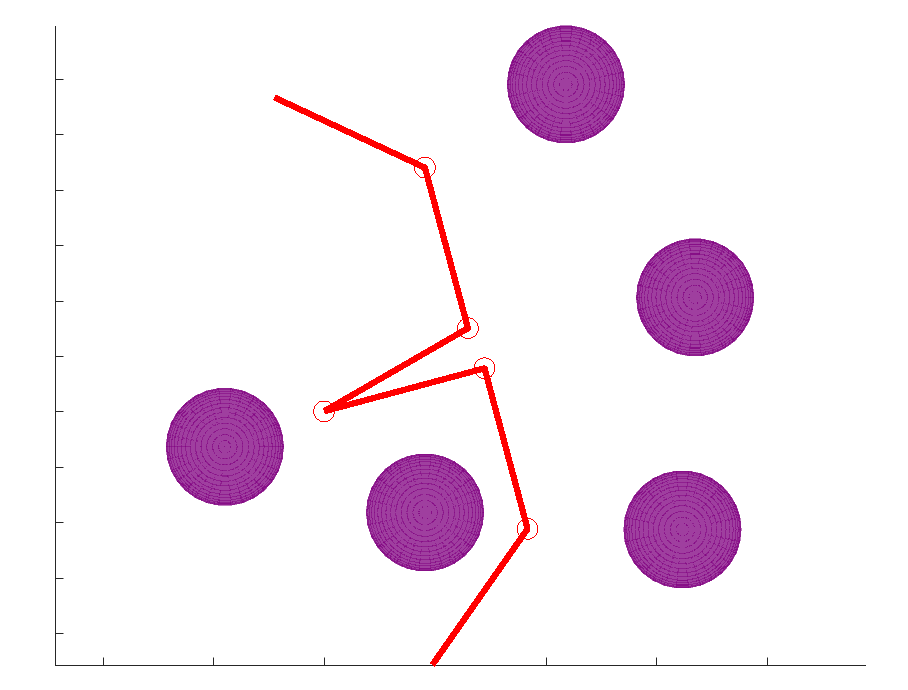
\includegraphics[width=0.2\textwidth]{Immagini/pdf/Problem_A_01.eps} \label{fig:Problem_A_01}} \quad
\subfloat[]{\includegraphics[width=0.2\textwidth]{Immagini/pdf/Problem_A_02.eps} \label{fig:Problem_A_02}} \\
\subfloat[]{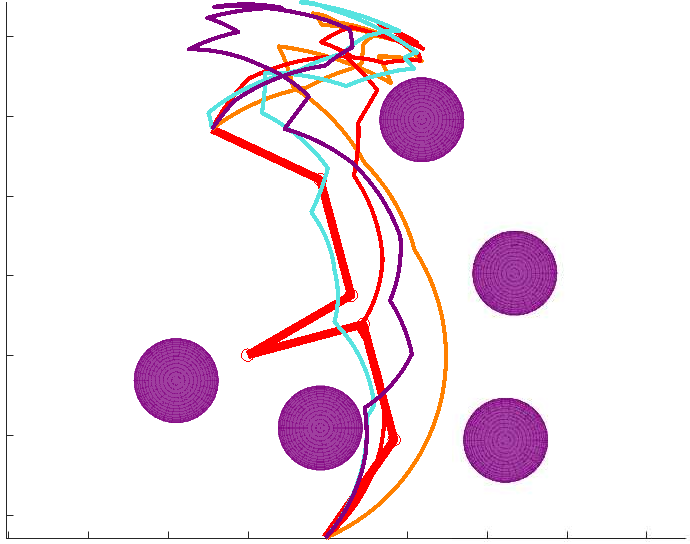
\includegraphics[width=0.2\textwidth]{Immagini/pdf/Problem_A_03.pdf} \label{fig:Problem_A_03}} \quad
\subfloat[]{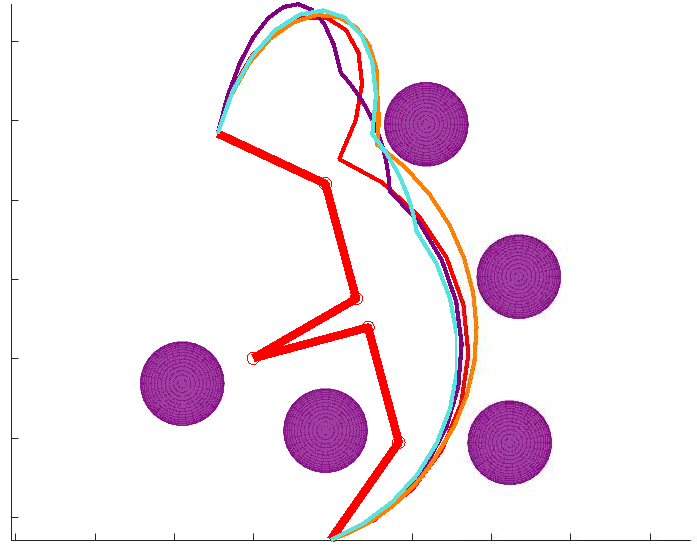
\includegraphics[width=0.2\textwidth]{Immagini/pdf/Problem_A_04.pdf} \label{fig:Problem_A_04}}
\caption{The two pictures on the top depict the planning problem considered for Problem 1. The purple spheres are the obstacles populating the workspace of the robot. On the left the poses $x_o$ and $x_f$, while on the right the optimal path obtained by applying RRT* with some intermediate poses and the trajectory of the E.E. 
The pictures at the bottom are examples of paths found when applying a standard (serial) RRT on the left; the multiagents version of RRT* described in Section \ref{subsec:MT_04} on the right.}
	\label{fig:Problem_1}
\end{figure}

\subsection{Problem 2 : path planning with a 7 d.o.f robot }
\label{sec:probl_2}

Another path planning problem is considered here, similar to the previous one and with the same workspace. 
However, here the robot considered, reported in Figure \ref{fig:Problem_2}, has 7 d.o.f. 
Notice that time $T_V$ is more than doubled with respect to Problem 1; while time $T_{\tau}$ is almost the same.    

\begin{figure}
	\centering
	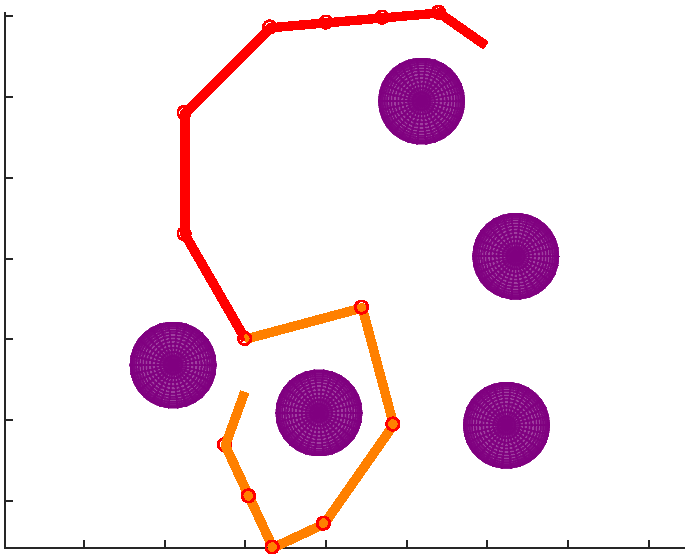
\includegraphics[width=0.2\textwidth]{Immagini/pdf/problem_7gdl.pdf} \label{fig:Problem_A_01}
\caption{The planning problem considered for Problem 2. The starting and ending poses of the robot are depicted respectively in red and in orange. }
	\label{fig:Problem_2}
\end{figure}

\subsection{Problem 3 : trajectory planning}
\label{sec:probl_3}

In this case, we consider the same scenario of Problem 1, but considering a trajectory planning problem.
The state $x$ is composed as follows:
\begin{eqnarray}
x=[ q^{T} \,\,\,\, \dot{q}^{T} ]^{T}
\end{eqnarray}
where $q$ is the pose of the robot (angular displacements), while $\dot{q}$ are the joint velocities. The second order minimum time trajectory connecting two states $x_{1,2}$ is considered as $\tau_{1 \rightarrow 2}$. Such a trajectory can be computed by making use of the Reflexxes library \cite{Reflexxes}, which takes into account the kinematic limitations of a manipulator, but not the obstacles populating the scene. The cost $C(\tau_{1,2})$ is assumed  as the time for reaching $x_2$ when following $\tau_{1,2}$. The states $x^{1,\cdots,K}_s$ considered by the steering function are separated by a (small) fixed time $\Delta t$: $x^{k}_s = \tau(k \Delta t)$.
Notice that for this case time $T_V$ is equal to the same when considering Problem 1, while time $T_{\tau}$ is significantly higher.

\subsection{Problem 4 : kinodynamic planning}
\label{sec:probl_4}

This benchmark considers an optimal control problem. Consider the following non linear dynamical system whose equation of motion is as follows:
\begin{eqnarray}
\dot{x} &=& f(x) + u \label{eq:motion_problem_4} \\  
f(x) &=& T^{-1} \cdot 
diag(-1-e^{- \alpha_{1} x_1^2}, \cdots, -1-e^{- \alpha_{6} x_6^2})
\cdot T \nonumber\\
\end{eqnarray}
where all coefficients $\alpha_{1,2,3,4,5,6}$ are $>0$, while $T$ is an orthogonal matrix.
The state-space considered for planning is clearly the state-space of the above dynamical system.
A trajectory $\tau_{1 \rightarrow 2}$ is obtained integrating eq. (\ref{eq:motion_problem_4}) forward in time, under the effect of the optimal linear regulator obtained considering a linearization of the system:
\begin{eqnarray}
\dot{x} &=& \left( f(x_1) -A x_1 \right) + A x + u \texttt{\,\,\, where \,\,\,} 
A= \frac{\partial{ f }}{\partial{ x }} \vert _{x_1}  \nonumber\\
u &=& \hat{u} + A(x_1 - x_2) - f(x_1) \nonumber\\
\hat{u} &=& K (x_2 - x) 
\end{eqnarray}
The gain matrix $K$ is computed such that:
\begin{eqnarray}
K = \underset{K}{\operatorname{argmin}}\left( \int_{0}^{\infty} \left( (x-x_2)^{T} Q (x-x_2) +  \hat{u}^{T} R \hat{u} \right) dt \right)
\end{eqnarray}
The steering function simply follows $\tau$ with fixed sample time.
The admissible region is structured as follows:
\begin{eqnarray}
x \in \underline{X} \Rightarrow  -2 & \leqslant  x_i   \leqslant & 2 \texttt{\,\,\,\,} 
\bigwedge \nonumber\\
 -5 & \leqslant  u_i(x)  \leqslant & 5  \texttt{\,\,\,\,}  \forall i=1,\cdots , 6 
\end{eqnarray}

%\begin{figure}
%	\centering
%\subfloat[]{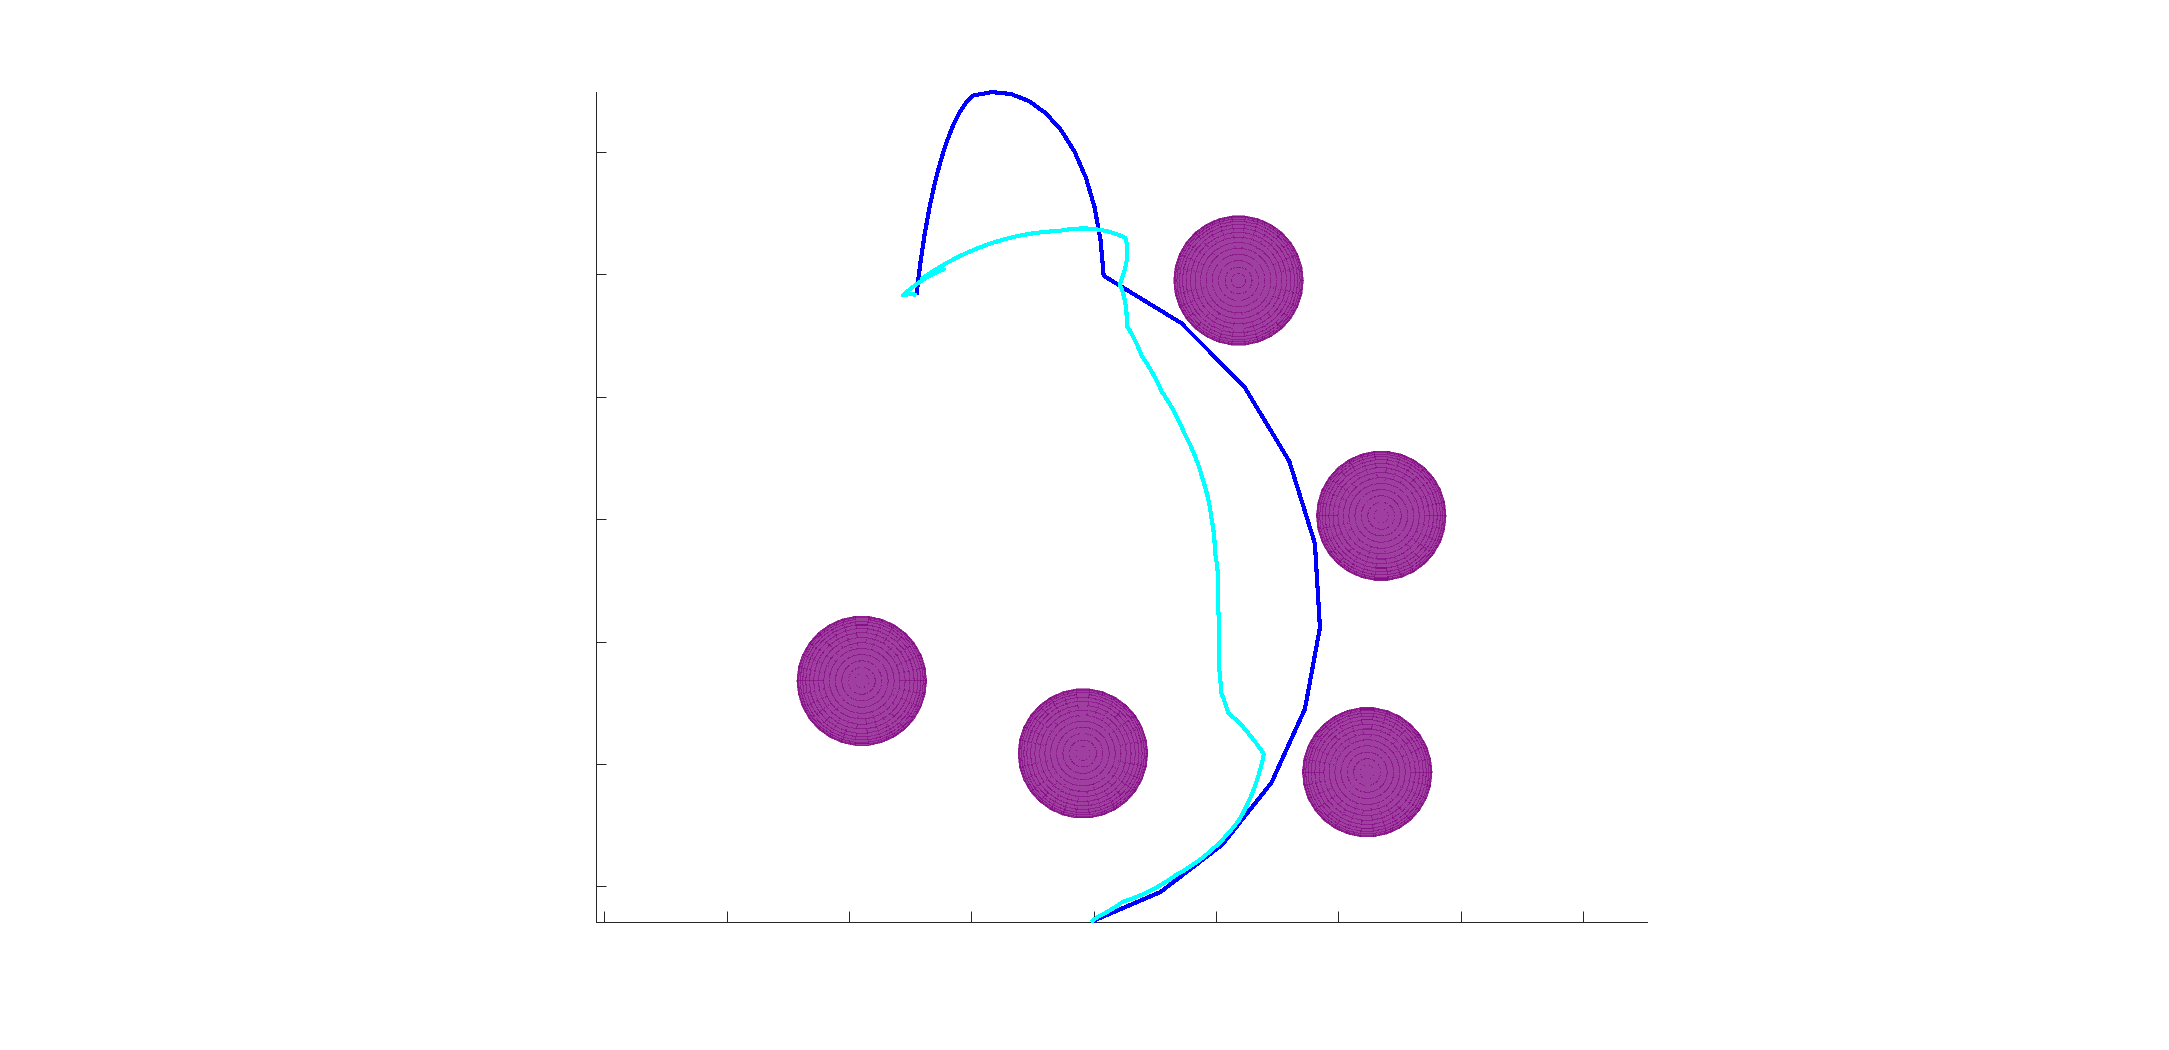
\includegraphics[width=0.2\textwidth]{Immagini/pdf/problem_B_01.eps}} \quad
%\subfloat[]{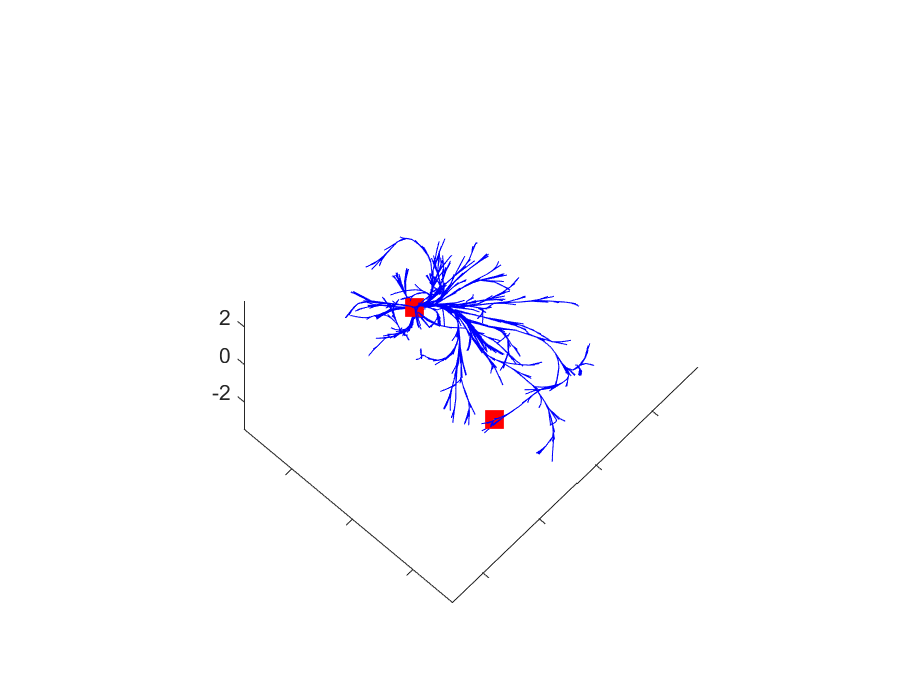
\includegraphics[width=0.2\textwidth]{Immagini/pdf/problem_B_02.eps}}
%\caption{On the left, the trajectory found by the RRT* algorithm as a solution to Problem B (cyan) in comparison to the solution found when considering a pure path planning problem (blue), i.e. problem A. On the right the tree obtained by the RRT* when solving problem B. METTERE spiegare perchè è diverso da path planning normale.}
%\end{figure}

\subsection{Results}

Figures \ref{fig:res_parall_query}, \ref{fig:res_shared}, \ref{fig:res_copied} and \ref{fig:res_ants} report the performance obtained when applying the strategies contained in MT-RRT, i.e. those described in Section \ref{sec:cap_03}, when varying the number of employed threads.
$\xi$ is the efficiency of the parallelization (normalized speed up, see \cite{efficiency_PC}), which is defined as follows (adopting the same notation of Section \ref{sec:cap_03}):
\begin{eqnarray}
\xi = \frac{T_{serial}}{T(P) \cdot P}
\end{eqnarray}
where $T_{serial}$ is the computation time absorbed by the standard serial versions presented in Section \ref{sec:cap_02}. In particular $T_{serial}$, was assumed as the mean value recorded for a batch of simulations. When having a good parallelization, $\xi$ should be close to 1 or higher. 
For all the simulations, the maximal number of iterations was set equal to 2500, and the termination criteria for all the versions adopting an RRT or a bidirectional RRT strategies was disabled: even in a case a solution was found, the search was not interrupted.
These results were obtained using a quad core laptop embedded with an Intel(R) core i7-6500u.

\begin{figure*}
	\centering
\subfloat[]{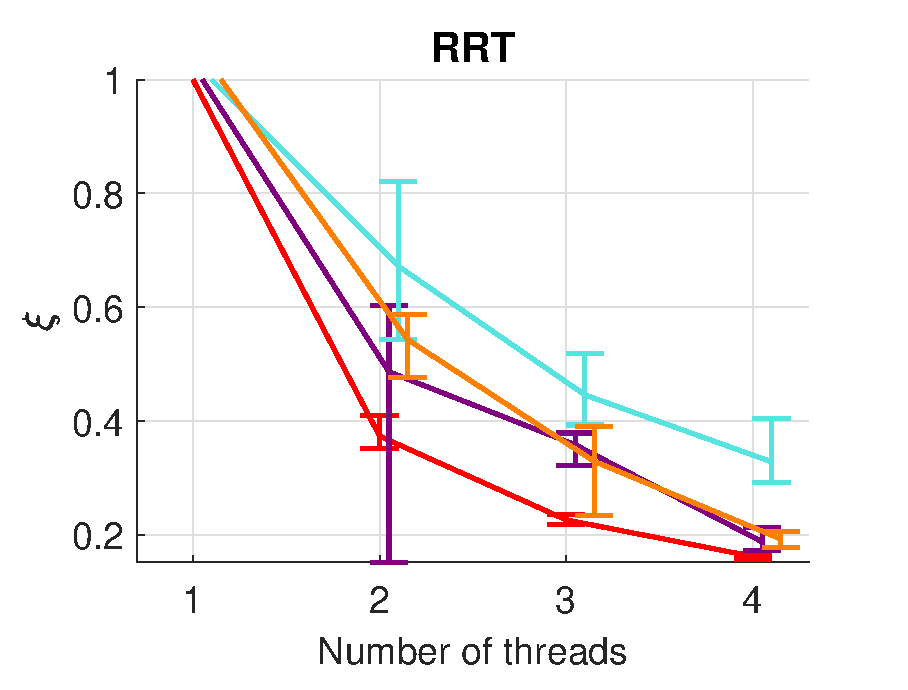
\includegraphics[width=0.31\textwidth]{Immagini/pdf/time_1_1.eps}} \quad
\subfloat[]{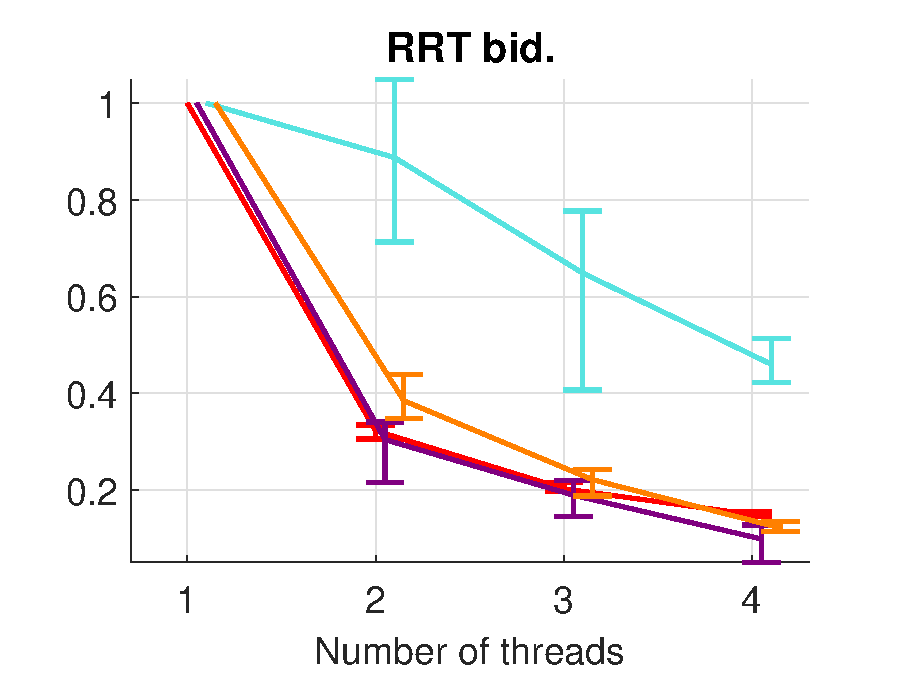
\includegraphics[width=0.31\textwidth]{Immagini/pdf/time_1_2.eps}} \quad
\subfloat[]{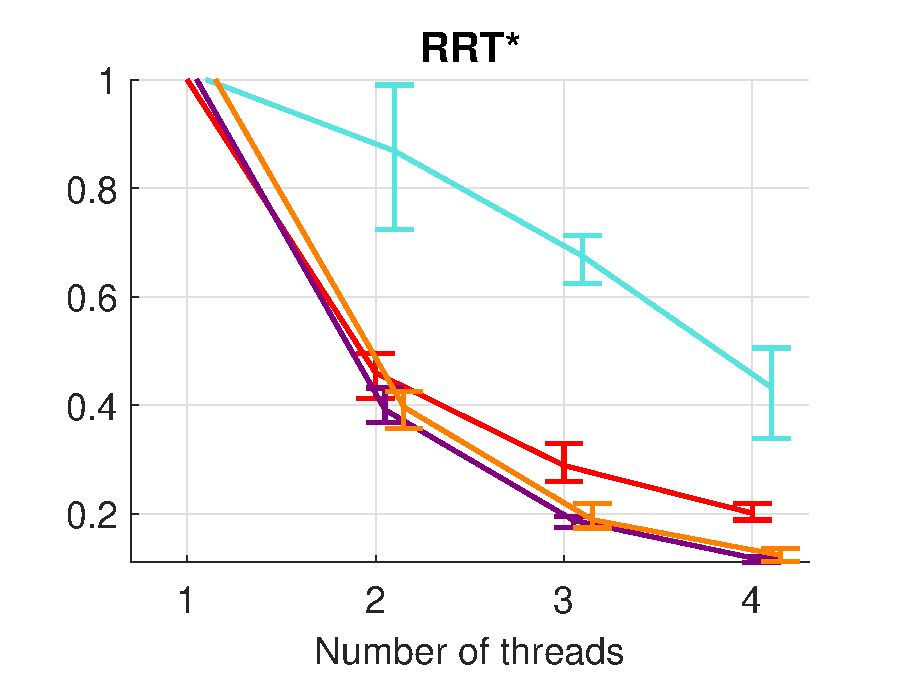
\includegraphics[width=0.31\textwidth]{Immagini/pdf/time_1_3.eps}} 
\caption{Performance obtained adopting the strategy described in Section \ref{subsec:MT_01}.}
\label{fig:res_parall_query}
\end{figure*}
\begin{figure*}
	\centering
\subfloat[]{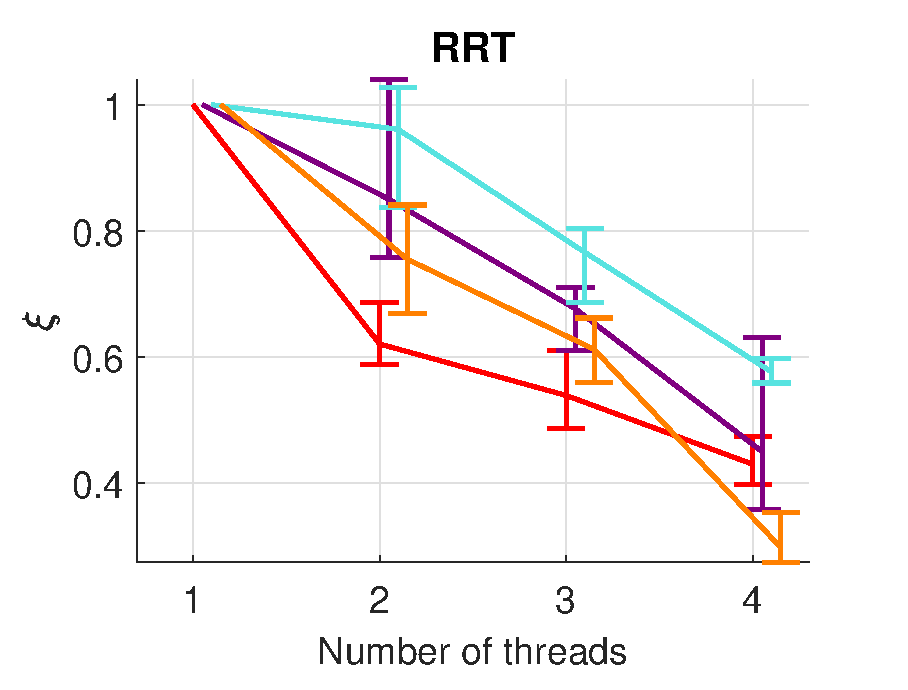
\includegraphics[width=0.31\textwidth]{Immagini/pdf/time_2_1.eps}} \quad
\subfloat[]{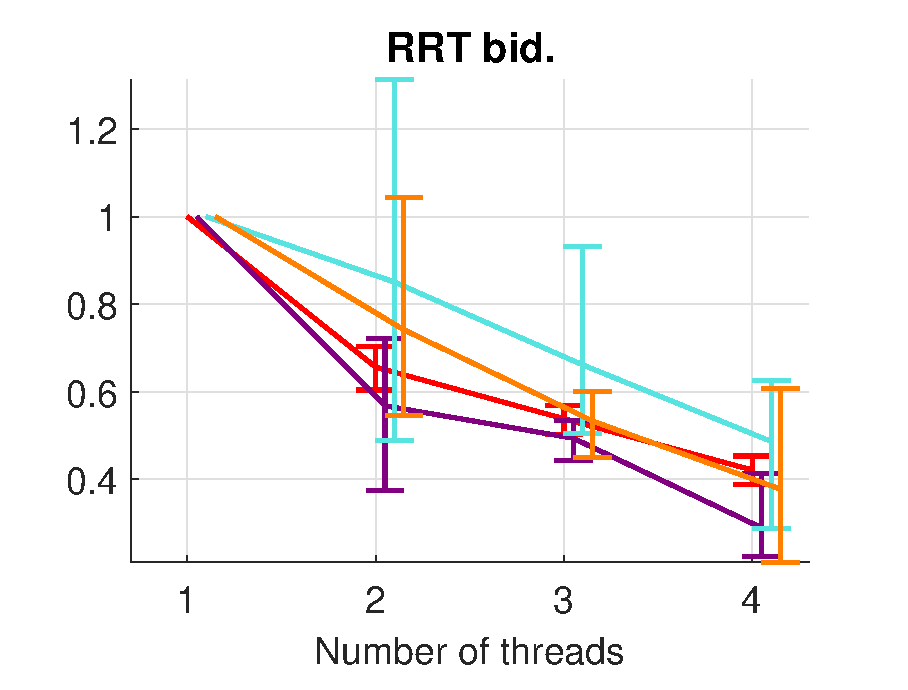
\includegraphics[width=0.31\textwidth]{Immagini/pdf/time_2_2.eps}} \quad
\subfloat[]{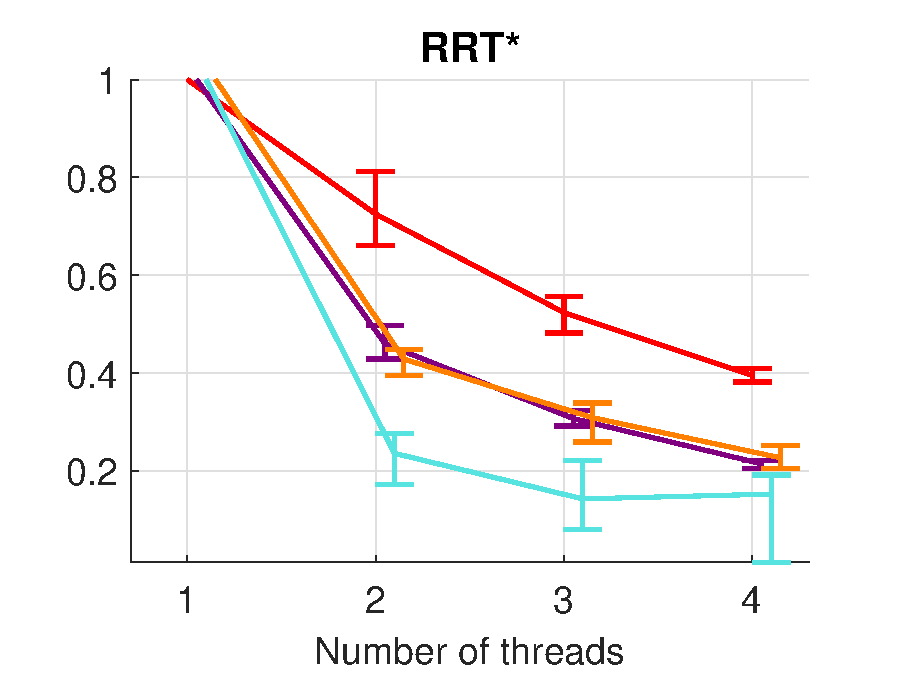
\includegraphics[width=0.31\textwidth]{Immagini/pdf/time_2_3.eps}} 
\caption{Performance obtained adopting the strategy described in Section \ref{subsec:MT_02}.}
\label{fig:res_shared}
\end{figure*}
\begin{figure*}
	\centering
\subfloat[]{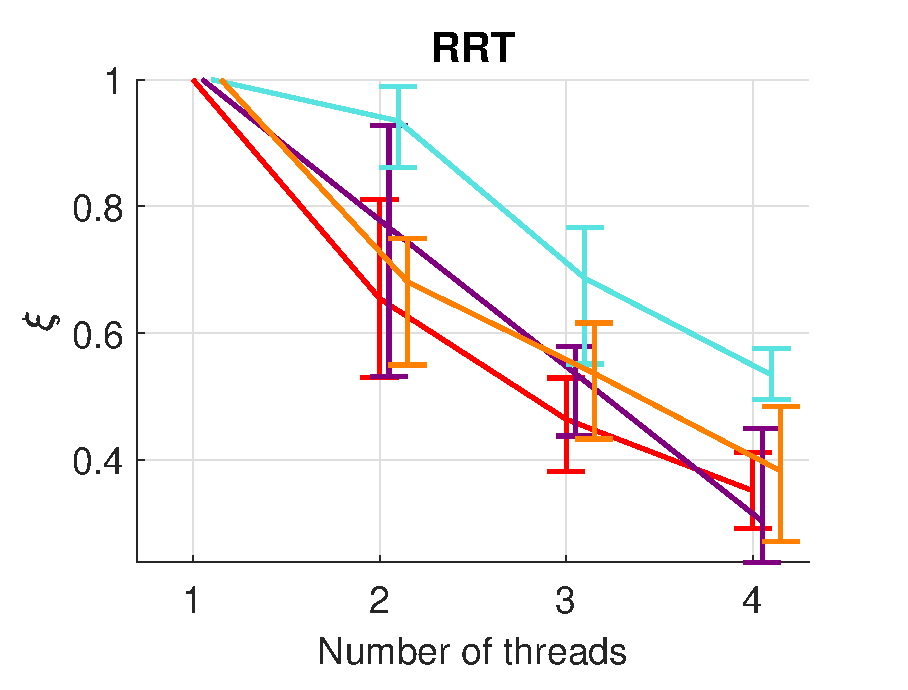
\includegraphics[width=0.31\textwidth]{Immagini/pdf/time_3_1.eps}} \quad
\subfloat[]{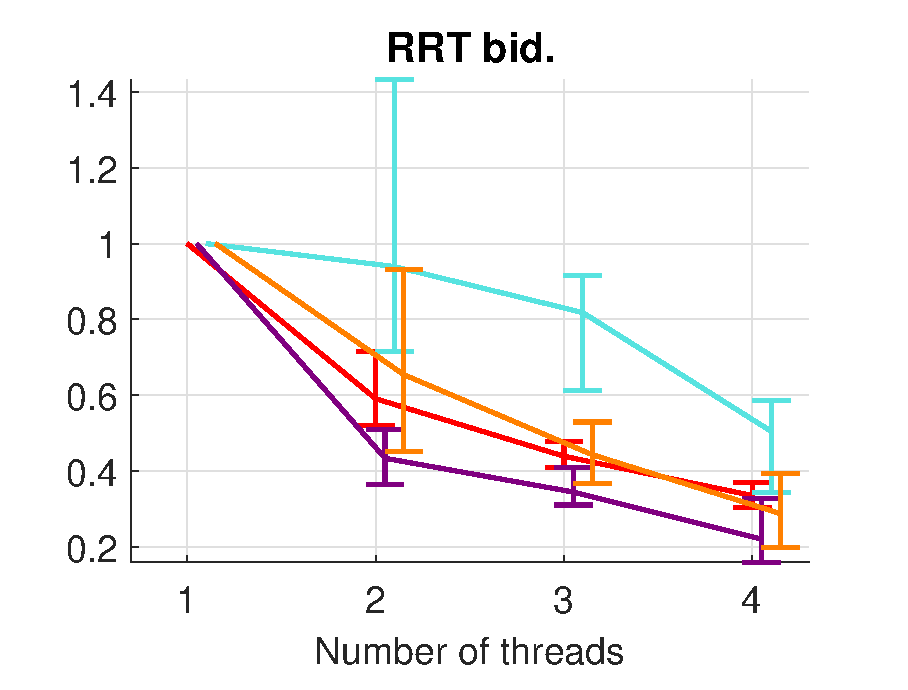
\includegraphics[width=0.31\textwidth]{Immagini/pdf/time_3_2.eps}} \quad
\subfloat[]{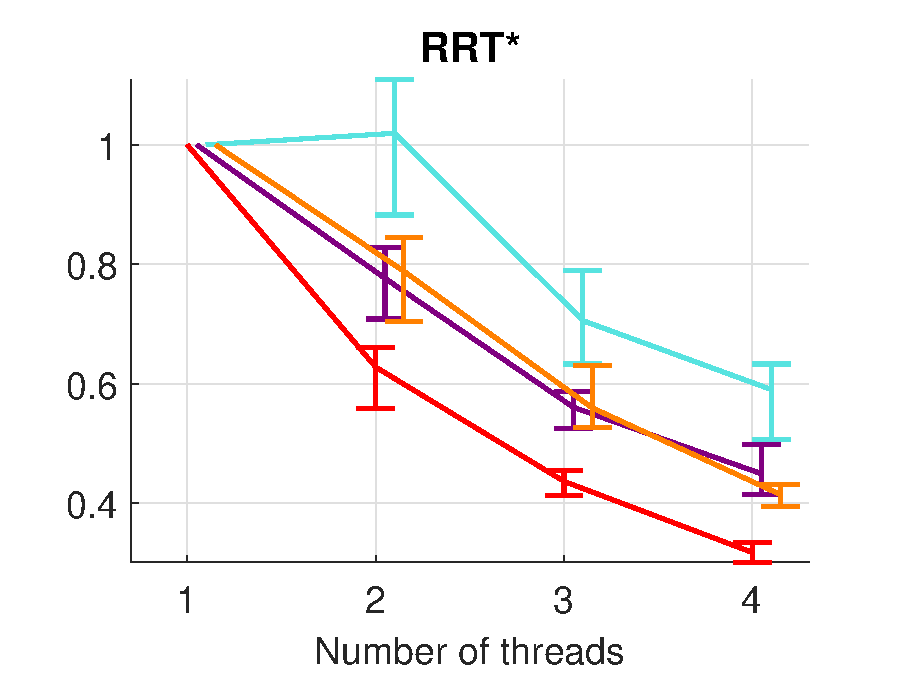
\includegraphics[width=0.31\textwidth]{Immagini/pdf/time_3_3.eps}} 
\caption{Performance obtained adopting the strategy described in Section \ref{subsec:MT_03}.}
\label{fig:res_copied}
\end{figure*}
\begin{figure*}
	\centering
\subfloat[]{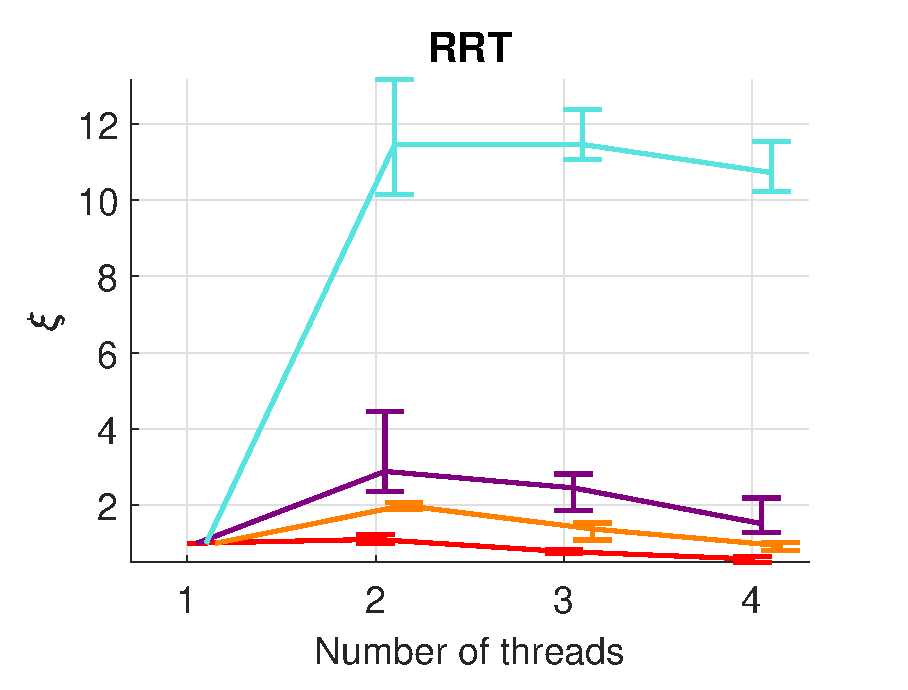
\includegraphics[width=0.31\textwidth]{Immagini/pdf/time_4_1.eps}} \quad
\subfloat[]{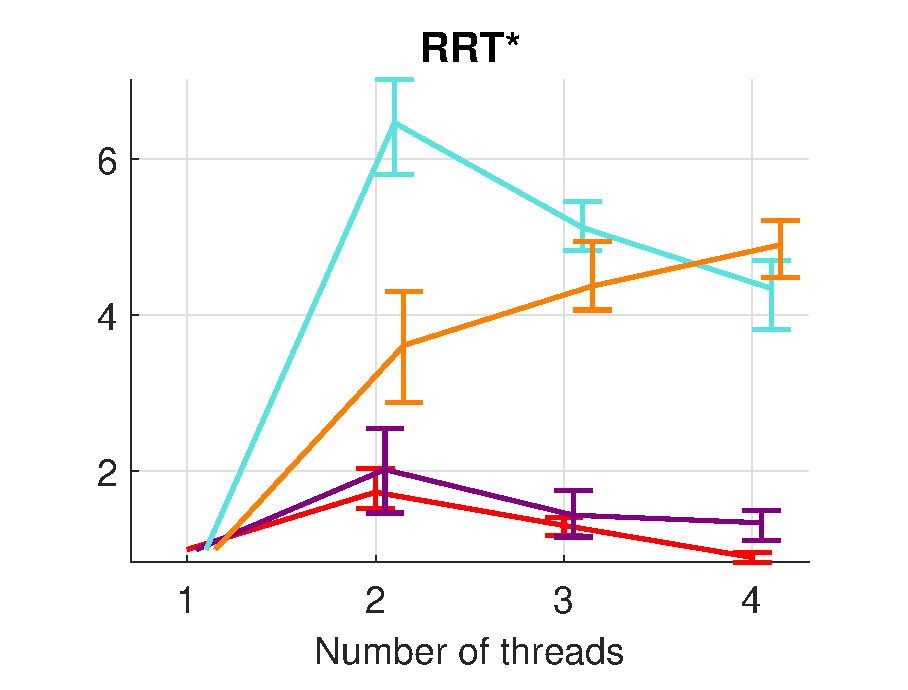
\includegraphics[width=0.31\textwidth]{Immagini/pdf/time_4_3.eps}} \quad
\subfloat[]{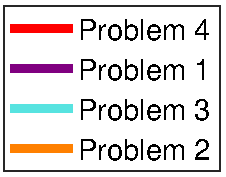
\includegraphics[width=0.15\textwidth]{Immagini/pdf/result_legenda.pdf}}
\caption{Performance obtained adopting the strategy described in Section \ref{subsec:MT_04}.}
\label{fig:res_ants}
\end{figure*}
